\documentclass[12pt,letterpaper]{article}

\usepackage{graphicx}
\usepackage{fancybox}
\usepackage[utf8]{inputenc}
\usepackage{epsfig,graphicx}
% \usepackage{multicol,pst-plot}
% \usepackage{pstricks}
\usepackage{amsmath}
\usepackage{amsfonts}
\usepackage{amssymb}
\usepackage{eucal}
\usepackage{upgreek}
\usepackage[left=2cm,right=2cm,top=2cm,bottom=1cm]{geometry}
\usepackage{tcolorbox}
\usepackage{import}
\pagestyle{empty}
\DeclareMathOperator{\tr}{Tr}
\renewcommand{\sp}[1]{$${\begin{split}#1\end{split}}$$}

\usepackage{lipsum}
\usepackage{mdframed}
\usepackage{listings}
\usepackage{color}

% Margins
% \topmargin=-0.45in
\evensidemargin=0in
\oddsidemargin=0in
\textwidth=6.5in
\textheight=9.0in
\headsep=0.25in

% \title{ Chemistry Notes}
% \author{ Gurmukh Singh }
% \date{\today}

 % The problem environment introduced.                                     
\newenvironment{problem}[2][Problem]                                  
        {\begin{tcolorbox}[colback=white,colframe=gray!50,title=#1 #2]}
        {\end{tcolorbox}}
        % {\begin{mdframed}[backgroundcolor=gray!20] \textbf{#1 #2} \\}
        % {\end{mdframed}}
% Define solution environment
\newenvironment{solution}                      
        {\begin{mdframed}\textit{Solution:} \\}
        {\end{mdframed}}
% Define an environments for proofs
\newenvironment{myproof} 
        {\textit{Proof:}}                                   
        {\begin{flushright} Q.E.D. \end{flushright}}
% Define a theorem environment and a notation one too
\newenvironment{mytheorem}                    
        {\begin{mdframed}\textbf{Theorem:} \\}
        {\end{mdframed}}
\newenvironment{notation}                      
        {\begin{mdframed}\textit{Notation:} \\}
        {\end{mdframed}}
% A new example wouldnt so any harm either...  
\newenvironment{example}                             
        {\textit{Example:}\\}
	{}
%I sholud be ashamed to forget the definition environment

\newenvironment{definition}
	{\begin{mdframed}$\underline{\textit{Def}^\textit{n}:} $\\}
	{\end{mdframed}}
%Corollary envvvvvvvvv
\newenvironment{corollary}
	{\textbf{Corrolary:}\\}

\pagestyle{empty}

\begin{document}

\begin{center}
  \Huge{Operating Systems}\\
  \vspace{0.25cm}
  \small{Gurmukh Singh}
\end{center}

\vspace{-1.75cm}

\begin{flushright}
  Instructor: \\ Mr. Amit Chauhan
\end{flushright}

\vspace{-1.3cm}

\begin{flushleft}
  B.Tech. CSE
\end{flushleft}

\rule{15.5cm}{0.1mm}%{\linewidth}{0.1mm}

% Optional TOC
\tableofcontents
\pagebreak

%--Paper--

\section{Operating systems}
\begin{definition}
  Operating system is an interface between user and the hardware.
  Without operating system the user cannot access any hardware. 
\end{definition}

\begin{definition}
   When we have many programs running at one given time, we need to allocate CPU to one of them and memory with osem other application. 
   This is known as resource sharing. Sometimes resources are not sharable so we allocate some process or program and later after taking it back we can allocate it to some other process. 
\end{definition}
 
\begin{enumerate}
  \item Operating system acts like a manager. It is a kind of book keeping like which resource is currently allocated to which process. 
  \item memory can be managed like : 
    \begin{itemize}
      \item how much memory do we have?
      \item how much memory we can allocate? 
      \item how much free memocy is available?
    \end{itemize}
\end{enumerate}

\subsection{Goals of operating systems: }
\begin{enumerate}
  \item Primary Goal : Convenience ( personal computers )
  \item Secondary Goal: Efficiency ( Supercomputers )
\end{enumerate}

\subsection{Types of operating systems:}
\begin{enumerate}
  \item Batch OS 
  \item Multiprogramming OS
  \item Multitasking OS
  \item Multiprocessing OS
  \item Real time OS
\end{enumerate}

\subsubsection{Batch OS}
There used to be a single computer to which everyone was given access. This computer is called mainframe and everyone should give a program to this mainframe computer in a queue.
Then the comuter will pick them one after the other and execute them and later at some point the user will pick the program.

If any of the jobs require less amount of CPU time  and more I/O time since here CPU time is greater than I/O time still CPU is not allocated to any other job until the current process is completed.
It is not interactive as well which means thatresponse is not given immediately

\subsubsection{Multiprogramming OS}
It is basically an extension to Batch processing using multiprogramming CPU will be used efficiently. e.g. suppose the first job requires I/O then it will go to I/O device then CPU will be allocated to second job at the same time in such a way that CPU remains busy as longer as the are jobs. 

Advantages of Multiprogramming OS:
\begin{enumerate}
  \item We need not to keep CPU ideal. 
  \item CPU will be busy all the time with maximum utilization
\end{enumerate}

\subsubsection{Multitasking OS}
It is an extension to multiprogramming OS. CPU will be multiplexing among all the jobs without completing any first job. 
Like for some time CPU is allocated to job1 then to job2 then to job3 and so on. And repeat this cycle again and again. 

e.g. round robin approach. 

\subsubsection{Multiprocessing OS}
In this instead of having one CPU we will be having lots of CPU's in the same computer. 

Advantages:
\begin{enumerate}
  \item Many jobs can be run simultaneously and parallelism can be achieved.
  \item Throughput can be improved. (number of jobs completed per unit time.)
  \item if one CPU fails, jobs can be rescheduled between other CPU's
\end{enumerate}

\subsubsection{Real time OS}
In this scenario, we are given some jobs and jobs will be having some deadlines. then we are supposed to finish those jobs in the assigned deadline. \\ 
In this scenario timing is everything. 

\section{Process management}
suppose we write a file ``exa.c" in C language. 
now the program has to be first converted from high level language to  low level language or machine language. This process is done by a compiler. 

Program generally resides in the secondary memory. Operating system will take it from secondary memory and place it in main memory. Then start the execution. 
When the OS puts the program in main memory, it creates a datastructure called a process. 

\subsection{Process}
It is something which is created by the operating sysetem in order to execute a program. So before we execute a program we need to create a process. The proces is real and the program is virtual. 

For example: Making of the food is the process and the recipie is the program

\begin{center}
  \import{Imports/}{Process.pdf_tex}
\end{center}

Once the Datastructure is created, the OS will start executing the executable code line by line. 

\subsubsection{Attributes of a process}

\begin{enumerate}
  \item Process ID 
  \item Program counter 
  \item Process state
  \item Priority 
  \item General purpose register
  \item List of open files 
  \item List of open devices 
  \item Protection
\end{enumerate} 

\textbf{Process ID:}\\
Each process is given a unique number called the process ID. the number of bits depends on the OS. 

\textbf{Program counter:}\\
While we are executing a process, we suddenly start a process and then we restart it at the end of execution. 

\textbf{Process state:}\\
This is the current state of the process. 

\textbf{Priority:}\\
Whenever a process is created by an OS, it is assigned some priority. So a process with high priority will be executed first by the CPU. 

\textbf{GPR:}\\
When a process is prempted and some other process comes for execution then the contents of the registers related to the prempted process should also be preserved so that when it resumes it's execution consistency will be maintained.

\textbf{List of open files:}\\
During the execution of a process some files need to be opened , some of the files are opened for reading purpose and others for writing purpose. 

\textbf{List of oped devices:}\\
Devices which are currently used by the process 

\textbf{Protection:}\\
One process should not go into other process workspace and vice versa. For every process OS is going to create a process control block (PCB) which stores all the above information about a process. 

\subsection{States of a process} 
A process from it's creation to completion. Depending upon the requirements a process will transition from one state to another. 
When we have a lot of processes that are ready to rum is known as multiprogramming. 


States of a process
\begin{enumerate}
  \item New: Whenever a process is created It is in the new state.
  \item Ready: whenever processes are created they are ready to run in the main memory. There are various processes which are ready to run
    In multiprogramming there are two types of processes: 
    \begin{enumerate}
      \item With premption\\
        (AKA multitasking or time sharing)
        With premption the process is forcefully stopped 
      \item Without premption\\
        Without premption the process is allowed to complete it's execution, it is not forced to stop.
    \end{enumerate}
  \item Run\\
    simultaneously only process will be running if we have one CPU and if we have $n$ CPU's then $n$ processes will be running simultaneously.
  \item Block/wait\\
    Sometimes a process which is running might need some resources like a file or access to a device then we pull it out and put it in block state or wait state until it finishes with I/O. Once it finishes the I/O we again bring it to previous state i.e. ready state.  
  \item Termination/completion\\
    Once a process finishes or completes it's execution it is known to be in completion stage or termination stage. Once a process completes it's execution it's PCB(Process control block) is also deleted. 
  \item Suspend ready\\
    Whenever space in main memory is not sufficient and whenever we want to accomodate more important processes(high priority processes) we just move the low priority processes out of the main memory to the secondary memory. 
    These are the set of processes which work initially in the ready state and now because of lack of resources we are throwing them outside into the secondary memory. 
  \item Suspend wait/ suspend block\\
    performing processes are performing some I/O and are waiting for initialization so we let them wait in secondary memory or move to wait or block state of secondary memory. 
\end{enumerate}

\subsection{Generation of OS:}
\begin{enumerate}
  \item First generation: (1940-1948)\\
    large and expensive.
  \item Second Generation: (1956-1963)\\
    transistors replaced vaccuum tubes\\
    generated a lot of heat. 
  \item Third Generation(1964-1971)\\
    Introduced IC. \\
    transistors were placed on silicon chips\\
    keyboards and monitors became widespread. 
  \item Fourth Generation(1971-present)\\
    Microprocessors, GUI's, mouse and handheld device.
  \item Fifth Generation(Present and beyond)\\
    Based on AI, Early stage\\
    voice recognition\\
    parallel processing and superconductors are aiding this transition.\\
    quantum computers and nanotechnology.
\end{enumerate}

\subsection{Services of OS:}
\begin{enumerate}
  \item provide programs an environment to execute. 
  \item provide users means to run programs. 
\end{enumerate}

\subsection{Program execution}
\begin{enumerate}
  \item leads a program into memory. 
  \item execution the program. 
  \item handles program's execuion. 
  \item Provides a mechanism for process syncronization.
  \item Provides a mechanism for process communication. 
  \item Provides a mechanism for deadlock handling. 
\end{enumerate}

\subsection{Operations on process}
\begin{enumerate}
  \item Creation:\\ Once a process is created it is in ready state and is present in main memory. 
  \item Scheduling\\ When we have many processes in the ready queue we schedule it and give it to the CPU i.e. allocate the CPU to one of them on the basis of Scheduling. 
    \begin{itemize}
      \item New state: Process is about to be created and it is currently present in the secondary memory. 
    \end{itemize}
  \item Executing:\\ Once we give a process to the CPU it will start the execution. 
  \item Killing/Delete:\\ Whenever we are done with the process we can simply kill the process. 
\end{enumerate}

\subsection{Process state transition Diagram}
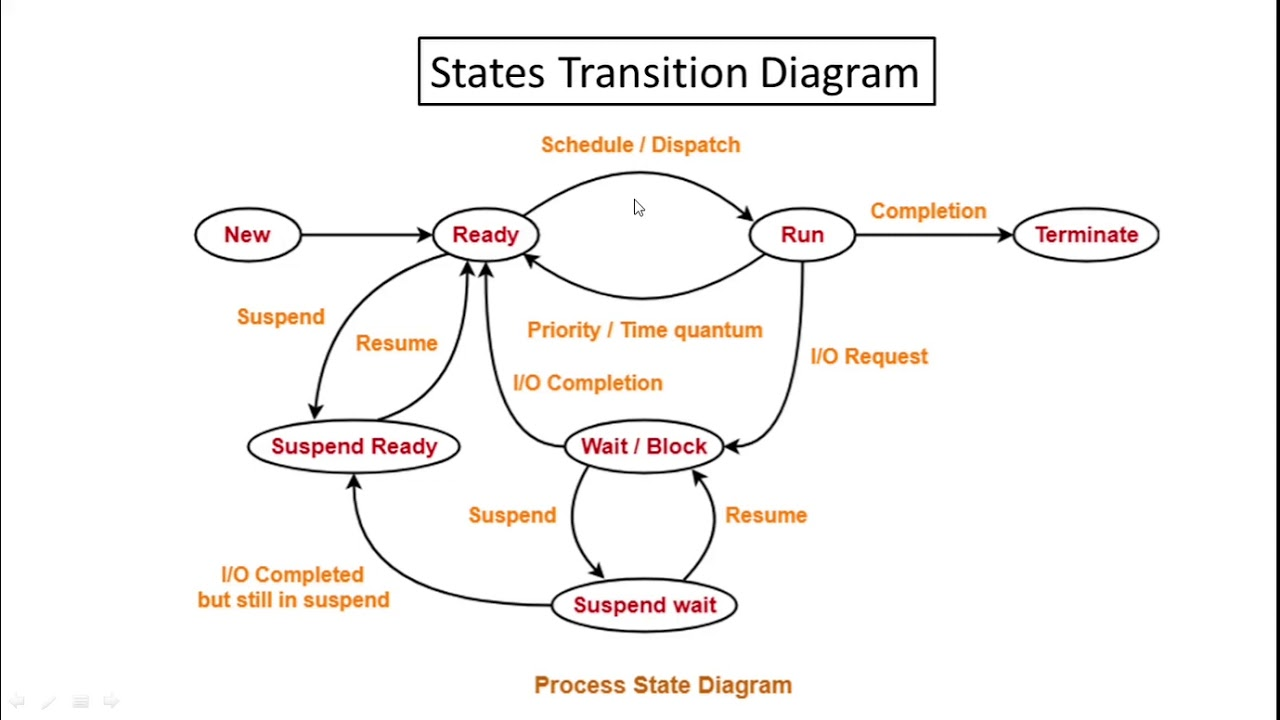
\includegraphics[width=\textwidth]{Imports/processstatetransition.png}
NOTE:\\
\begin{itemize}
  \item The minimum number of states a process can go through is 4. (New, Ready, Run, Terminate)
  \item Priority or time quantum may cause a process to premp
  \item Suspend wait or suspend ready are in secondary memoryare in secondary memory.
  \item I/O can occur anywhere (in main memory as well as in secondary memory) without any interruption once it is initiated. 
\end{itemize}

\subsection{Types of Schedulars in OS}
There are 3 types of Schedulars in OS: 
\begin{enumerate}
  \item Long term Schedular:\\ Long term Schedular is responsible for the decisions about how many processes have to be created. 
  \item Short term schedular:\\ Once we have a pool of processes waiting in ready queue to be alloted to CPU for execution. This decision is taken by short term scheduler AKA dispatcher.
  \item Medium term scheduler:\\ Suspension decisions are taken by Medium term scheduler. this decision can be taken either in ready state or in wait or block state. 
\end{enumerate}

NOTE:\\
Long term decisions of how many processes to be created is also known as degree of multiprogramming. (Number of processes that are present in the ready queue at maximum)

When the processes are present in the states, they're basically presented as queues. These queues are implemented as linked lists. 
\vspace{1cm}

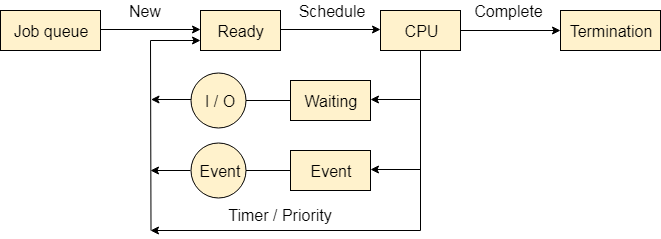
\includegraphics[width=0.8\textwidth]{Imports/ProcessQueue.png}\\
fork() command is used for creating a new process and that process will go to the ready queue. 

\subsection{Various times related to processes}
\begin{enumerate}
  \item Arrival time: \\ Whenever a process gets in the ready queue it is the time at which the process is ready for execution.
  \item Burst time: \\ The amount of CPU time required by a process to finish (hard to predict/detect) in real time. 
  \item Completion time: \\ The time at which the process completes it's execution is called completion time.
  \item Turn around Time: \\ Completion time and arrival time are basically points in time whereas waiting time and burst time are durations in time. In between arrival time and completion time we can have a process 
    either waiting or executing. The difference between completion time and arrival time is called Turn around time.
  \item Waiting time: \\ The difference between Turnaround Time and Burst time is called Waiting time. 
  \item Response time: \\ What is the first time the process hits the CPU after it arrives. 
\end{enumerate}

\subsection{CPU Scheduling:}
Picking up a process from the ready queue and giving it to the CPU is called CPU scheduling. The short term scheduler will perform CPU scheduling. 
\begin{itemize}
  \item Who $\rightarrow$ short term scheduler 
  \item Where $\rightarrow$ Ready state to running 
  \item When $\rightarrow$ When a process moves
\end{itemize}

\subsection{Scheduling algorithms}
FCFS(First Come First Serve): 
\begin{itemize}
  \item if two processes have the same arrival time then pick the one with lower process numbers. 
\end{itemize}
Note: one disadvantage of FCFS is convey effect (convey: when a process is having large burst time then all the processes which are greater will have to starve. This is also known as starvation process)

SJF(Shortest job first):
\begin{itemize}
	\item Criteria: burst time 
	\item Mode: Non premption
\end{itemize}
Whichever process has the least burst time is executed first. The process is not stopped until it is finished.
Whenever two processes have the same burst time pick the one which has arrived earlier. SJF is the best known scheduling algorithm as of now.
Advantages:
\begin{itemize}
	\item maximum throughput
	\item minimum average waiting time.
\end{itemize}
Disadvantages:
\begin{itemize}
	\item Starvation to longer jobs.
	\item It is not implemented because burst time of processes cannot be known as ahead \end{itemize}
Throughput is maximum at any point of schedule for SJF because we complete as many jobs as possible depending upon test burst time.

\end{document}
